%
% kurve.tex -- Kurve 
%
% (c) 2021 Prof Dr Andreas Müller, OST Ostschweizer Fachhochschule
%
\documentclass[tikz]{standalone}
\usepackage{amsmath}
\usepackage{times}
\usepackage{txfonts}
\usepackage{pgfplots}
\usepackage{csvsimple}
\usetikzlibrary{arrows,intersections,math,calc}
\definecolor{darkred}{rgb}{0.8,0,0}
\definecolor{darkgreen}{rgb}{0,0.6,0}
\begin{document}
\def\skala{1}
\begin{tikzpicture}[>=latex,thick,scale=\skala,
declare function={
	X(\t) = 0.04*cos(\t)*\t;
	Y(\t) = sin(\t);
	X0(\t) = \t;
	Y0(\t) = 0.3*\t;
	X1(\t) = \t;
	Y1(\t) = -0.1*\t;
	g1x(\t) = 0.1*\t*\t;
	g1y(\t) = 0.2*\t*\t;
	g2x(\t) = 0.1*\t*\t*\t-0.1*\t*\t;
	g2y(\t) = -0.2*\t*\t;
}]

\begin{scope}[xshift=-7.4cm]

	\begin{scope}[xshift=0.4cm,yshift=-4.3cm]
		\draw[->] (-1.5,0) -- (1.5,0);
		\draw[line width=1.2pt] (-0.6,0) -- (0.6,0);
		\node at (-1.5,0) [above] {$\mathbb{R}$};
		\node at (1.5,0) [above] {$x^1$};
		\node at (-0.5,0) [above] {$U$};
		\fill (0,0) circle[radius=0.05];
		\node at (0,0) [below] {$\psi(x)$};

		\draw[->,color=darkred] (1.8,0.4) to[out=10,in=170] (4.2,0.4);
		\node at (3,0.6) [above] {$\varphi\circ\gamma_1\circ\psi^{-1}$};
		\draw[->,color=blue] (1.8,-0.4) to[out=-10,in=-170] (4.2,-0.4);
		\node at (3,-0.6) [below] {$\varphi\circ\gamma_2\circ\psi^{-1}$};
	\end{scope}

	\draw[line width=1.4pt]
		plot[domain=-40:80,samples=100] ({X(\x)},{Y(\x)});
	\fill ({X(10)},{Y(10)}) circle[radius=0.05];
	\node at ({X(10)},{Y(10)}) [above left] {$x$};
	\node at ({X(80)},{Y(80)}) [left] {$X$};

	\draw[->,shorten <= 0.2cm] ({X(10)},{Y(10)}) -- ++(0.0,-4.0);
	\node at ($({X(10)},{Y(10)})+(0,-2)$) [left] {$\psi$};

	\begin{scope}[xshift=0.4cm]
		\draw[->,color=darkred]
			(1.8,0.6) to[out=10,in=170] (4.2,0.6);
		\node[color=darkred] at (3,0.8) [above] {$\gamma_1$};
		\draw[->,color=blue]
			(1.8,-0.2) to[out=-10,in=-170] (4.2,-0.2);
		\node[color=blue] at (3,-0.4) [below] {$\gamma_2$};
	\end{scope}
\end{scope}

\begin{scope}[yshift=0.25cm]

	\node at (0,-0.2) {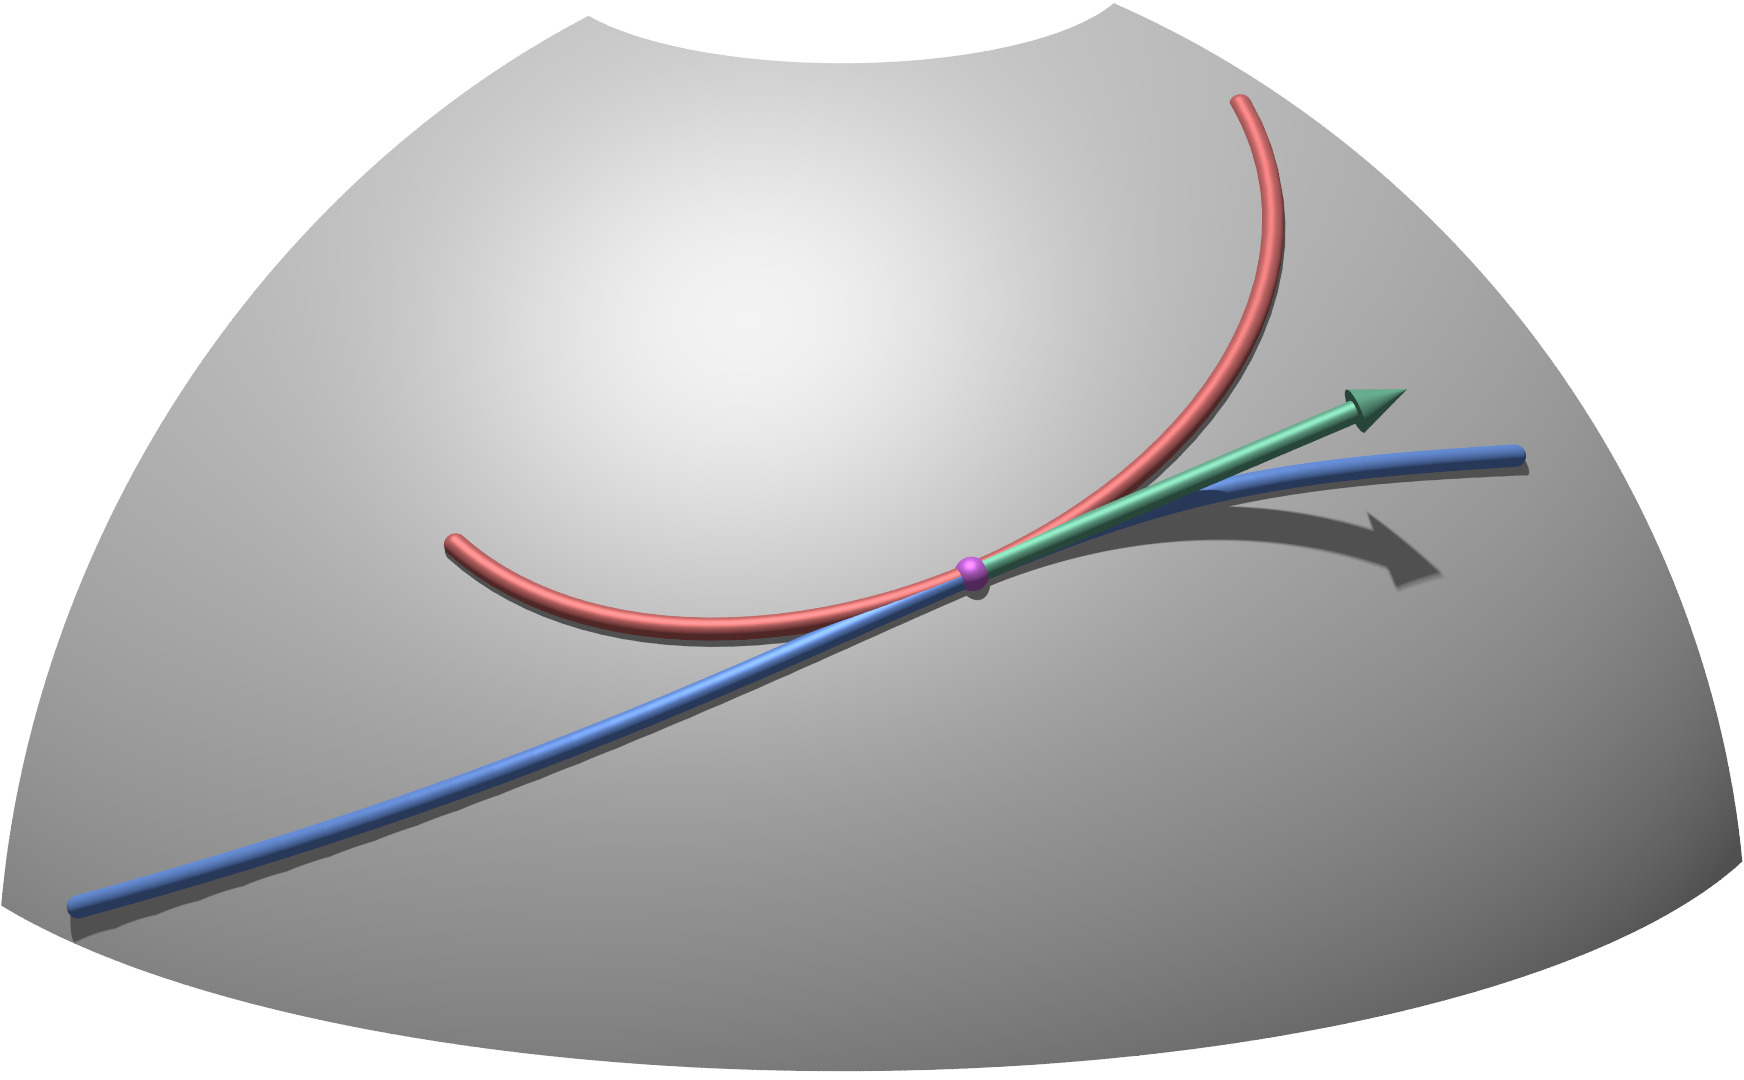
\includegraphics[width=4.8cm]{kurve.jpg}};
%	\fill[color=gray!40,rounded corners=0.5cm]
%		(-2.5,-1.5) rectangle ++(5,3);
	\node at (-0.8,1.0) {$Y$};
%
%	\draw[->,color=darkgreen,line width=1.2pt]
%		(0,0) -- ++({X0(1.5)},{Y0(1.5)});
%	\draw[color=darkred,line width=1.4pt]
%		plot[domain=-1.5:1.5,samples=100]
%			({X0(\x)+g1x(\x)},{Y0(\x)+g1y(\x)});
%	\draw[color=blue,line width=1.4pt]
%		plot[domain=-1.5:1.5,samples=100]
%			({X0(\x)+g2x(\x)},{Y0(\x)+g2y(\x)});
%	\fill[color=violet] (0,0) circle[radius=0.08];
	\node[color=violet] at (0.2,-0.3) [above] {$y$};


	\draw[->] (0,-1.7) -- ++(0,-2.6);
	\node at (0,-3.0) [right] {$\varphi$};

	\begin{scope}[yshift=-4.6cm]
		\draw[->,color=darkgreen,line width=1.2pt]
			(0,0) -- ++({X1(1.5)},{Y1(1.5)});
		\draw[color=darkred,line width=1.4pt]
			plot[domain=-1.5:1.5,samples=100]
				({X1(\x)+g1x(\x)},{Y1(\x)+g1y(\x)});
		\draw[color=blue,line width=1.4pt]
			plot[domain=-1.5:1.5,samples=100]
				({X1(\x)+g2x(\x)},{Y1(\x)+g2y(\x)});
		\fill[color=violet] (0,0) circle[radius=0.08];
		\draw[->] (-2.4,-1.1) -- (2.4,-1.1)
			coordinate[label={$y^1$}];
		\draw[->] (-1.5,-1.2) -- (-1.5,1.2)
			coordinate[label={left:$y^n$}];
	\end{scope}
\end{scope}


\end{tikzpicture}
\end{document}

